\documentclass[11pt,a4paper]{article}
\usepackage[T1]{fontenc}
\usepackage{graphicx,isabelle,isabellesym}
\usepackage{amssymb}

% for \<guillemotright>
\usepackage[english]{babel}

% this should be the last package used
\usepackage{pdfsetup}

% urls in roman style, theory text in math-similar italics
\urlstyle{rm}
\isabellestyle{it}


\begin{document}

\title{Tycon: Type Constructor Classes \\ and Monad Transformers}
\author{Brian Huffman}
\maketitle

\begin{abstract}

These theories contain a formalization of first class type constructors and axiomatic constructor classes for HOLCF. This work is described in detail in the ICFP 2012 paper ``Formal Verification of Monad Transformers'' by the author \cite{huffman2012}. The formalization is a revised and updated version of earlier joint work with Matthews and White \cite{HMW05}.

Based on the hierarchy of type classes in Haskell, we define classes for functors, monads, monad-plus, etc. Each one includes all the standard laws as axioms. We also provide a new user command, \emph{tycondef}, for defining new type constructors in HOLCF.  Using \emph{tycondef}, we instantiate the type class hierarchy with various monads and monad transformers.

\end{abstract}

\tableofcontents

\begin{center}
  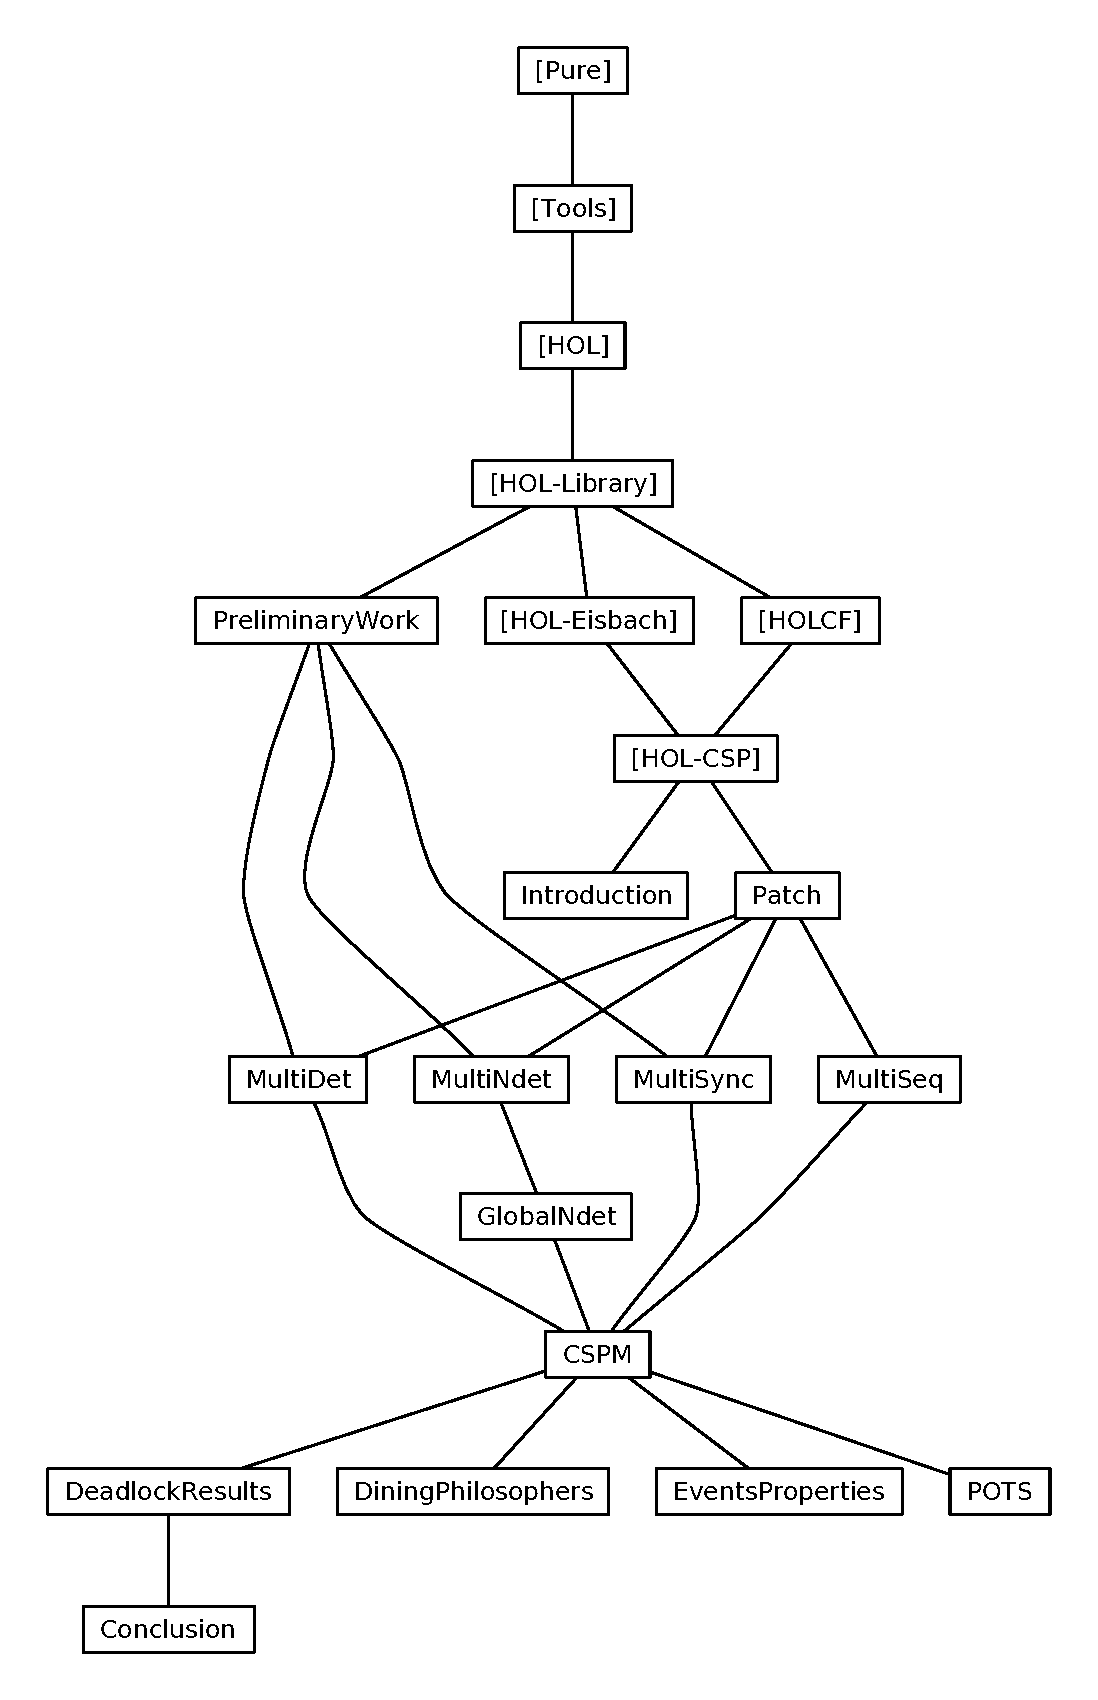
\includegraphics[width=\textwidth,height=\textheight,keepaspectratio]{session_graph}
\end{center}

\newpage

% use vertical space instead of indenting paragraphs
\parindent 0pt
\parskip 0.9ex

% include generated text of all theories
\input{session}

\bibliographystyle{abbrv}
\bibliography{root}

\end{document}
